% 本文件是示例论文的一部分
% 论文的主文件位于上级目录的 `bachelor.tex` 或 `master.tex`

\chapter{工作}

\section{公平性研究}
公平性问题是指,不同车辆通过同一个路口的通行时间可能有很大的差别,因为信号灯可能为了提高整体通行效率而牺牲一些车辆,让这些车辆多等待一些时间,即便这些车辆可能是先进入路口的,这对这些车来说是不公平的。一个好的控制策略应该在提高通行效率的同时能够保证每辆车所需的通行时间大致相同,也就是说,车辆通行时间的方差应该越小越好。但是已有的工作都是使用车辆的平均通行时间来衡量通行效率,很自然的忽略了公平性问题。
\subsection{目标}
本工作的目的是在提高通行效率(最小化平均通行时间)的同时,希望每条车道能够有尽可能相同的服务延迟(得到放行所需的时间)。这个目标可以用以下的Jain Fairness Index(JFI)指标来量化:
\begin{align}
    \mathcal{J} = \frac{(\sum_{i=1}^{M}\overline{D}_i)^2}{M\sum_{i=1}^{M}\overline{D}_i^2},
\end{align}
其中$\overline{D}_i$是第$i$条进近车道的平均延迟。当且仅当每一个$\overline{D}_i$都相等时,这个指标达到最大值,即是$1$。所以我们的目标也就是最大化这个指标。

\subsection{智能体设计}
\subsection*{状态表示}
在$t$时刻的状态$S(t)$由以下几个部分组成:
\begin{enumerate}
\item 交通流量:$\boldsymbol{V}(t)=\{V_1(t),V_2(t),\cdots,V_M(t)\}$。其中 $V_i(t)$表示第$i$条进近车道上车的数量。值得注意的是,由于右转不受限于信号灯的特殊性,这里我们不考虑右车道的交通流量。
\item 平均吞吐量:$\boldsymbol{\overline{L}}(t)=\{\overline{L}_1(t),\overline{L}_2(t),\cdots,\overline{L}_M(t)\}$。其中$\overline{L}_i(t)$表示第$i$条进近车道的平均吞吐量。同上,不考虑右车道的平均吞吐量。
\item 信号相位:$\boldsymbol{P}(t)$是当前信号相位的数字化表示,$1$表示绿色,可以通行;$0$表示红色,禁止通行。
\end{enumerate}
所以$S(t)=\{\boldsymbol{V}(t) || \boldsymbol{\overline{L}}(t) || \boldsymbol{P}(t) \}$
\subsection*{动作选择}
在本文中,动作选择机制是每次选择即将转换的信号相位。之后,交通信号灯将转换到这一新的相位并持续$\Delta t$的时间。为了安全起见,我们在两个不同的信号相位之间插入了3秒的黄色信号和2秒的红色信号。如果新选择的相位和当前相位相同,则不插入黄色和红色信号,以确保交通流畅。
\subsection*{奖励函数}
受PFS分配原则的启发,我们设计了一个可以在效率和公平之间提供良好的平衡的奖励函数,如下所示:
\begin{align}
\label{eq:reward}
    r = -\sum_{i=1}^{M} \frac{Q_i(t)}{\overline{L}_i(t) + \delta},
\end{align}
其中$Q_i(t)$ 和 $\overline{L}_i(t)$ 分别是第$i$条进近车道的队列长度和平均吞吐量。在每一次调度后(这里,我们将一次动作选择视作一次调度),$\overline{L}_i(t)$ 按照以下方式进行更新:
\begin{align}
    \overline{L}_i(t) = (1-\frac{1}{W})\overline{L}_i(t-1) + \frac{1}{W}L_i(t),
\end{align}
其中$L_i(t)$是此次调度中车道$i$上得到放行的车的数量,$W$是一个平衡通行效率和公平性的参数。另外,为了避免公式\ref{eq:reward}的分母为0, 我们加上了一个可以忽略不计的正数$\delta$。
\subsection*{训练过程}
训练过程伪代码如下:

\section{通信问题研究}
对于多路口的交通信号调度问题,协作(Coordination)可以有效地提升整体通行效率,以下列出几种常见的协作策略:
\begin{table}[htb]
    \caption[协作策略]{常见的协作策略\label{tab:coordination}}
    \begin{tabular}{clp{0.4\columnwidth}}
      \toprule
      协作策略 & 目标 & 说明 \\
      \midrule
      Global single agent & $max_{\mathbf{a}}Q(s, \mathbf{a})$ & $s$是全局的环境状态,$\mathbf{a}$是所有路口的联合动作。\\
      Independent RL without Communication & $max_{a_{i}}\sum{i}Q_{i}(o_i, a_i)$ & $o_i$是路口$i$的局部观测,$a_i$是路口$i$的动作。\\
      Independent RL with Communication & $max_{a_i}\sum{i}Q_i(\Omega(o_i, \mathcal{N}_i), a_i)$ &$\mathcal{N}_i$是路口$i$的邻近路口的状态表示,$\Omega(o_i, \mathcal{N}_i)$是整合路口$i$及其邻近路口状态表示的函数。\\
      \bottomrule
    \end{tabular}
\end{table}

\subsection{图神经网络}
\subsubsection{分类及介绍}
深度网络的研究推进了模式识别和数据挖掘领域的发展。借助于计算资源的高速发展(如GPU),深度学习在欧几里得数据(如图像、文本和视频)中取得巨大的成功。但是在一些应用场景下,数据(图)是由非欧几里得域生成的,任然需要有效分析。
例如,在电子商务领域,一个基于图的学习系统能够利用用户和商品之间的交互以实现精准的推荐。在化学领域,分子被建模为图,新药研发需要测定其生物活性。在论文引用网络中,论文之间通过引用关系互相连接,需要将它们分成不同的类别。

图数据的复杂性对现有机器学习算法提出了巨大的挑战,因为图数据是不规则的。每张图大小不同、节点无序,一张图中的每个节点都有不同数目的邻近节点,使得一些在图像中容易计算的重要运算(如卷积)不能再直接应用于图。此外,现有机器学习算法的核心假设是实例彼此独立。
然而,图数据中的每个实例都与周围的其它实例相关,含有一些复杂的连接信息,用于捕获数据之间的依赖关系,包括引用、朋友关系和相互作用。最近,越来越多的研究开始将深度学习方法应用到图数据领域。受到深度学习领域进展的驱动,研究人员在设计图神经网络的架构时借鉴了卷积网络、循环网络和深度自编码器的思想。

图神经网络的概念最早由Gori\cite{gori2005new}等人提出,由Scarselli\cite{scarselli2008graph}等人进一步阐明。早期的初期是以迭代方式通过循环神经网络架构传播邻近信息来学习目标节点的表示,直至达到稳定的状态。


图神经网络可以分为:图卷积网络(Graph Convolution Network),图注意力网络(Graph Attention Network),图自编码器(Graph Auto-encoder),图生成网络(Graph Generative Network)和图时空网络(Graph Spatial-Temporal Network)。
图卷积网络

图注意力网络是将注意力机制引入到基于空间域的图神经网络。图神经网络不需要使用拉普拉斯等矩阵进行复杂的计算,仅通过邻居节点的表征来更新目标节点的特征。由于能够放大数据中最重要部分的影响,注意力机制已经广泛应用到很多基于序列的任务中,图神经网络也受益于此,在聚合过程中使用注意力整合多个模型的输出。

图自编码器是一类图嵌入方法,其目的是利用神经网络将图的顶点表示为低维向量。典型的解决方案是利用多层感知机作为编码器来获取节点嵌入,其中解码器重建节点的邻域统计信息,如positive pointwise mutual information (PPMI)或一阶和二阶近似值。

图生成网络的目标是在给定一组观察到的图的情况下生成新的图。图生成网络的许多方法都是特定于领域的。例如,在分子图生成中,一些工作模拟了称为SMILES的分子图的字符串表示。在自然语言处理中,生成语义图或知识图通常以给定的句子为条件。

图时空网络同时捕捉时空图的时空相关性。时空图具有全局图结构,每个节点的输入随时间变化。例如,在交通网络中,每个传感器作为一个节点连续记录某条道路的交通速度,其中交通网络的边由传感器对之间的距离决定。图形时空网络的目标可以是预测未来的节点值或标签,或者预测时空图标签。最近的研究仅仅探讨了GCNs的使用,GCNs与RNN或CNN的结合,以及根据图结构定制的循环体系结构。

\subsubsection{应用分类}
以图结构和节点特征信息作为输入,根据输出的类别,可以将GNN的分析任务分为以下几类:
节点级别:这一类聚焦于节点回归和节点分类任务
边级别:
图级别:


使用GAT来学习communication,这样做有一下两个好处:
1. 动态学习周边的路口的重要性:已有的工作直接将目标路口及其邻近路口的状态直接整合起来,这种做法实际上是默认每一个邻近路口对目标路口的影响力是相同的。实际上由于交通在时间和空间上的变化,
同一个路口对于其目标路口的影响力也会发生变化。
2. 免索性模型学习(Index-free modeling learning):在多智能体场景下,通常需要使用参数共享(Parameter Sharing)来降低学习难度,从而加速学习。但是这一点在多路口信号控制场景下是不适用的,
因为不同路口对其邻近路口的敏感性是不同的。例如,如下图所示,有A,B两个路口,A对其N-S方向的交通更加敏感,B对其W-E方向的交通更加敏感,如果直接将A的参数分享给B,会导致B学习到的策略并不适用于
自身的场景。
\begin{figure}[htb]
  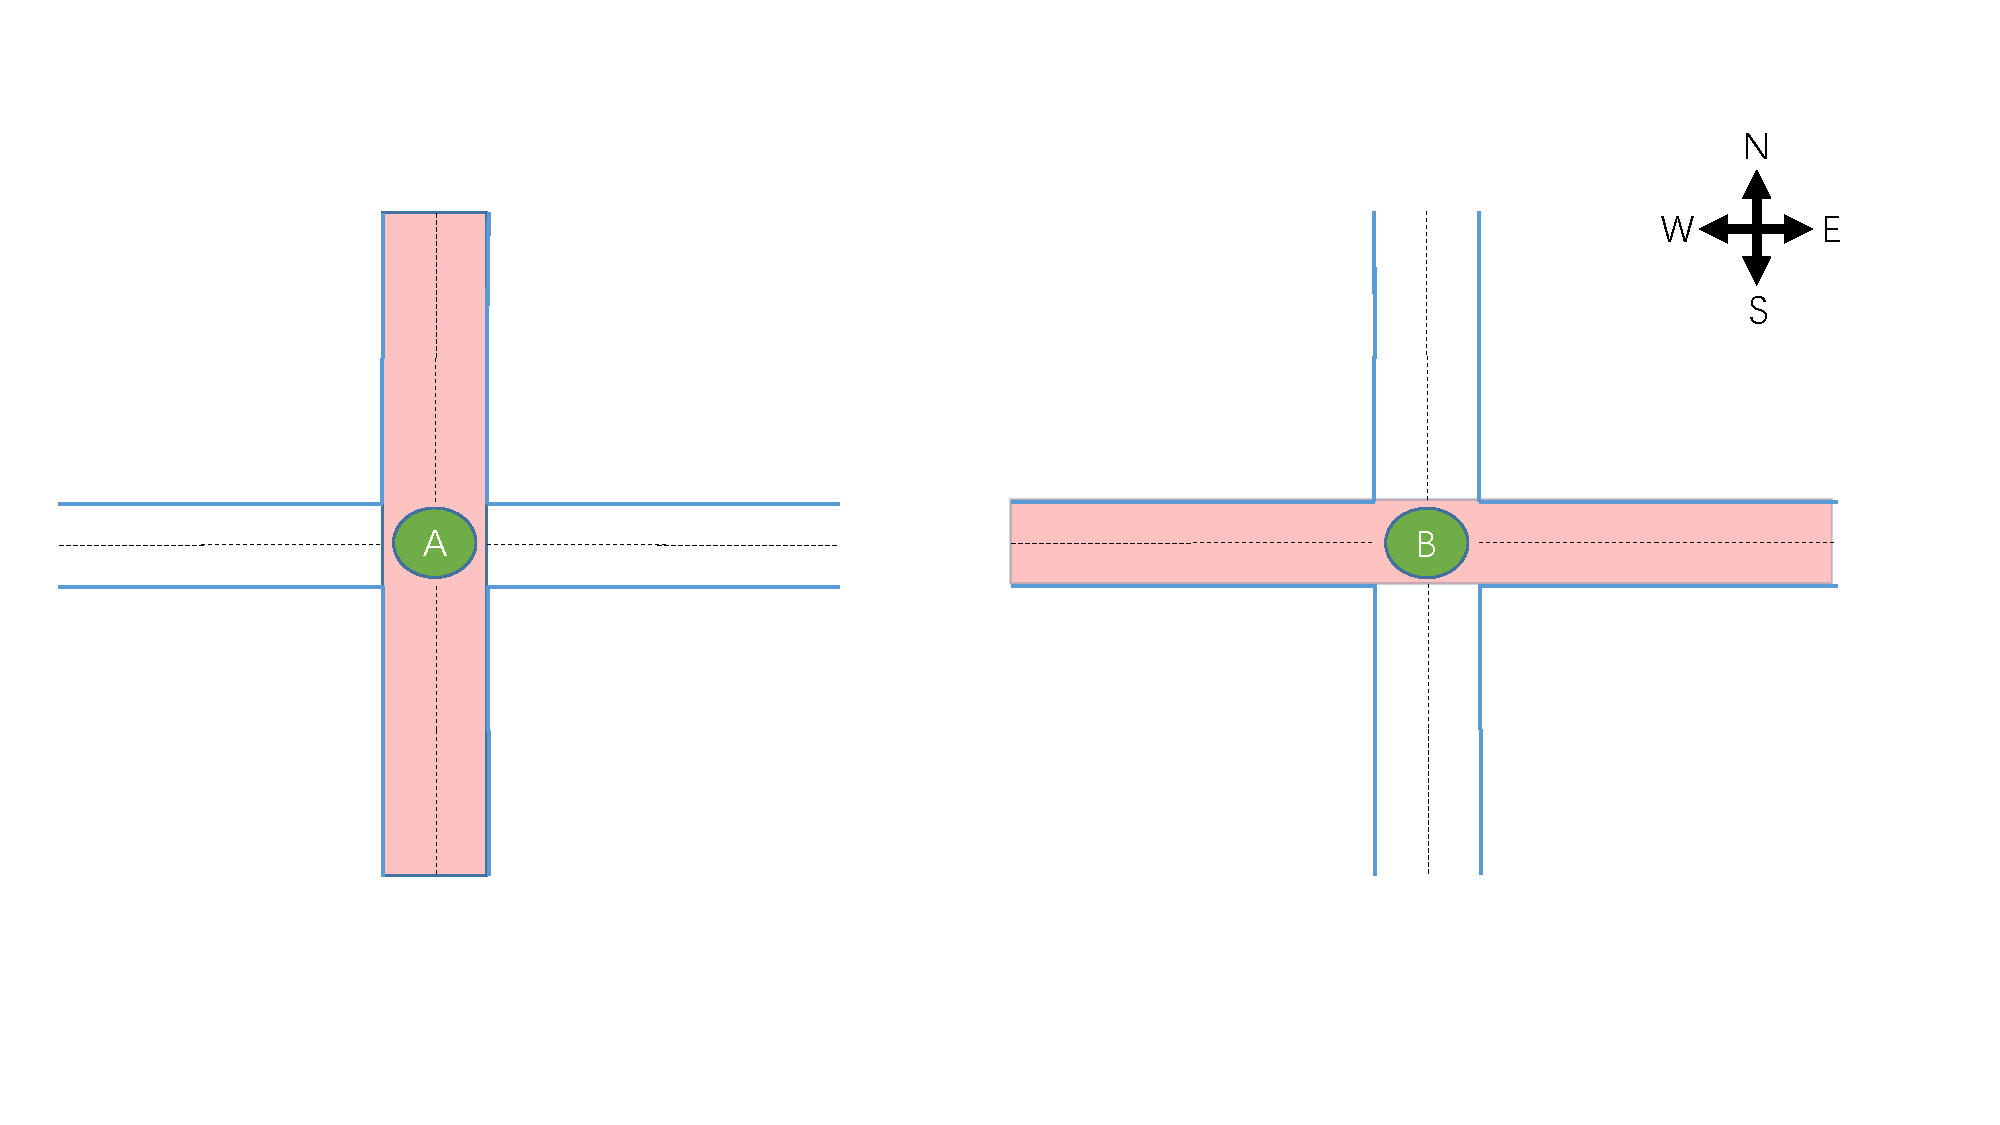
\includegraphics[width=10cm]{ppt/index-free.pdf}
  \caption{路口敏感性说明}
  \label{fig:index-free}
\end{figure}

使用IRL with communication的方法确实可以有效的解决维度灾难的问题。
已有的工作使用图神经网络来学习“交流”这一个过程。他们将每一个路口视作图中的一个节点,每条道路作为连接两个节点的边,很自然地可以将一张交通道路网建模成一个图。这种按路口建模的方式如下所示:
\begin{figure}[htb]
  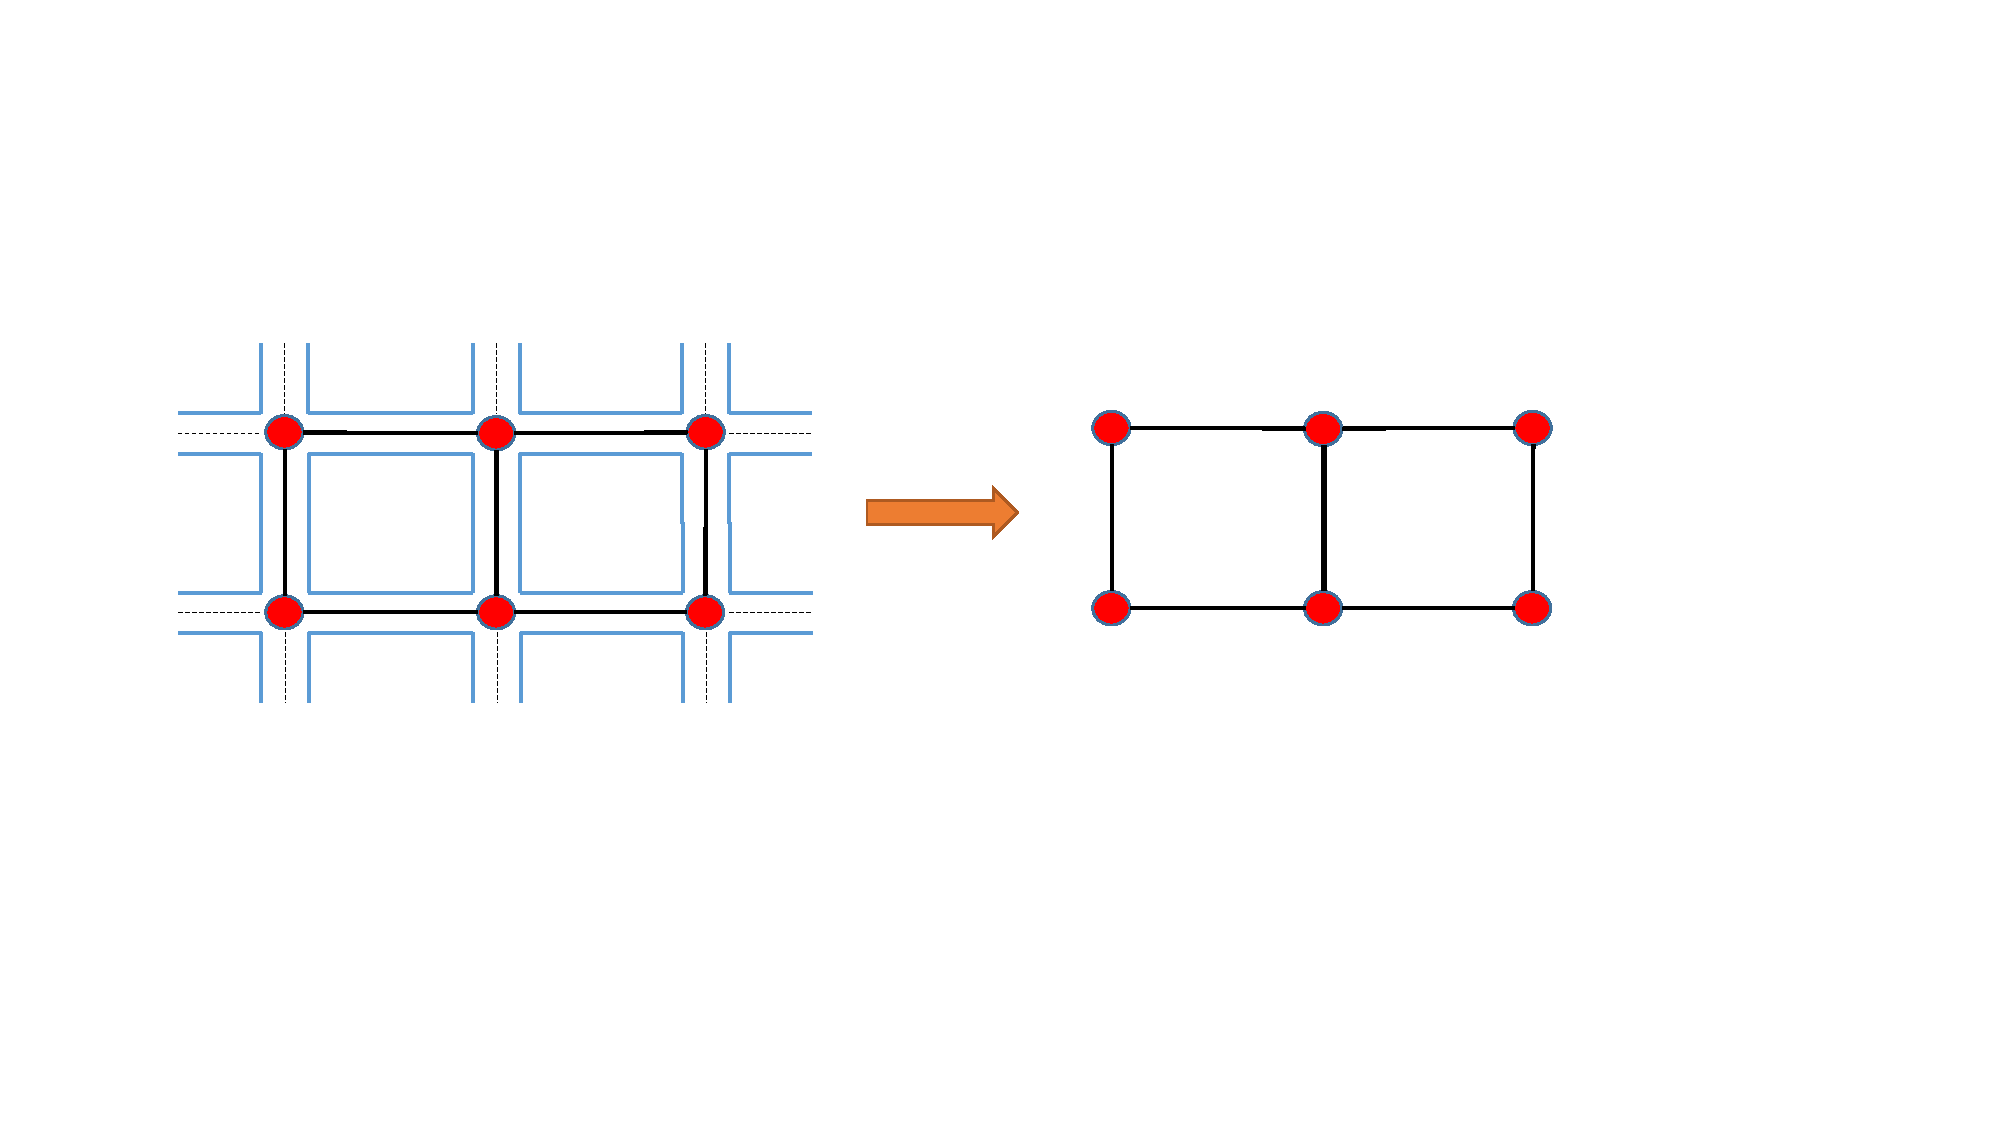
\includegraphics[width=10cm]{ppt/network-graph.pdf}
  \caption{多路口建模成图(路口)}
  \label{fig:network-graph-old}
\end{figure}

在这种建模方式下,每条车道的车辆以及当前的相位将作为该节点的特征。这种建模方式虽然可以很清晰的将多路口场景变成一张图。但是,因为是以一个路口为一个节点,所有车道的状态信息都整合到了一起,有些车道的的信息对目标节点是无用的,
如下图所示:
\begin{figure}[htb]
  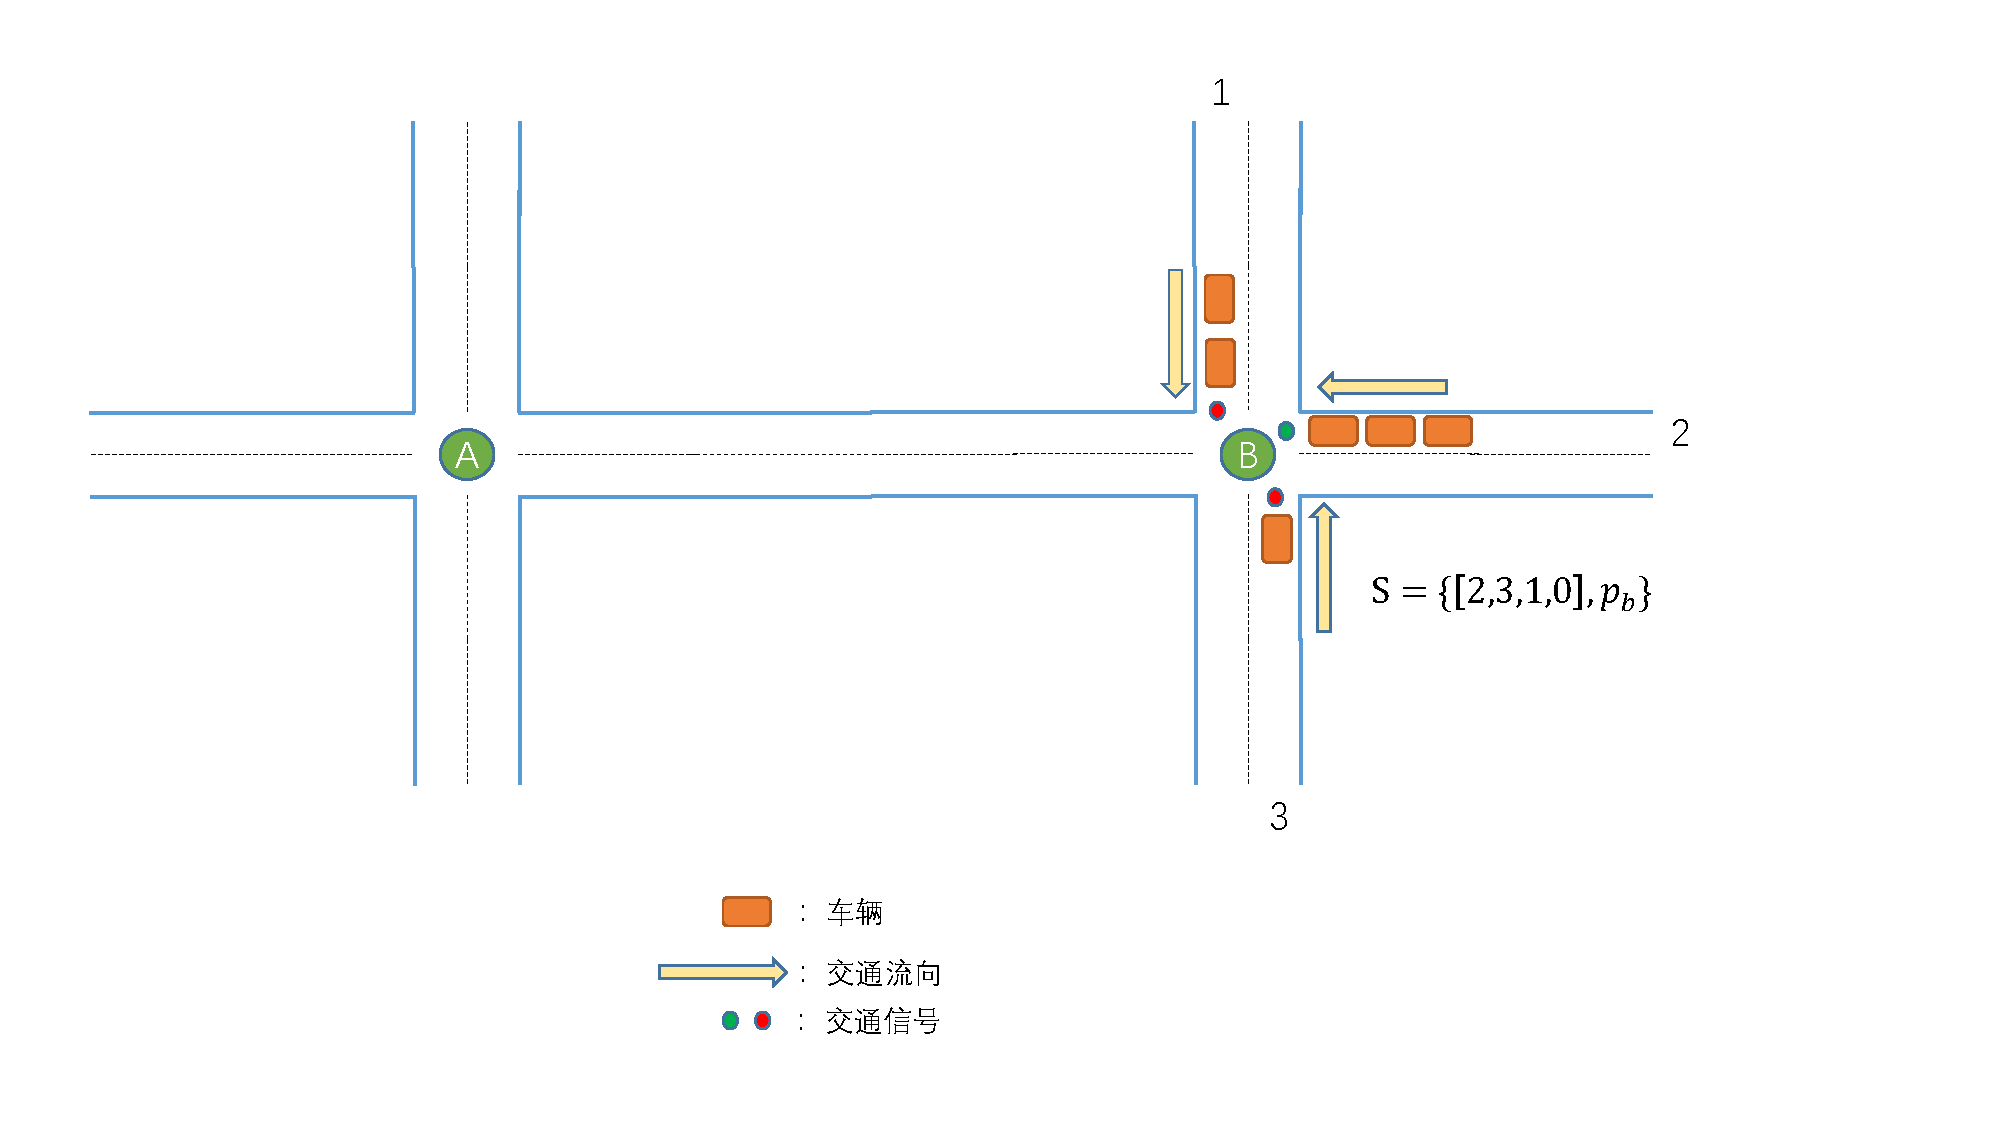
\includegraphics[width=12cm]{ppt/information-redundancy.pdf}
  \caption{按路口建图模式下信息传递}
  \label{fig:information-redundancy}
\end{figure}

路口B中只有2车道的交通流向与A车道有关,1、3车道的车辆不会行驶到A路口。在信息传递的时候,如果将所有的信息都笼统地传递过去,将会增加A提取有效信息的难度,从而降低学习的效率。

此外


在本文中,我们采用GAT来学习communication,不同的时,我们采用不同的图建模方式。我们不是按照路口来建图,而是按照道路来进行建模,即一条道路就是一个节点,如下图所示:
\begin{figure}[htb]
  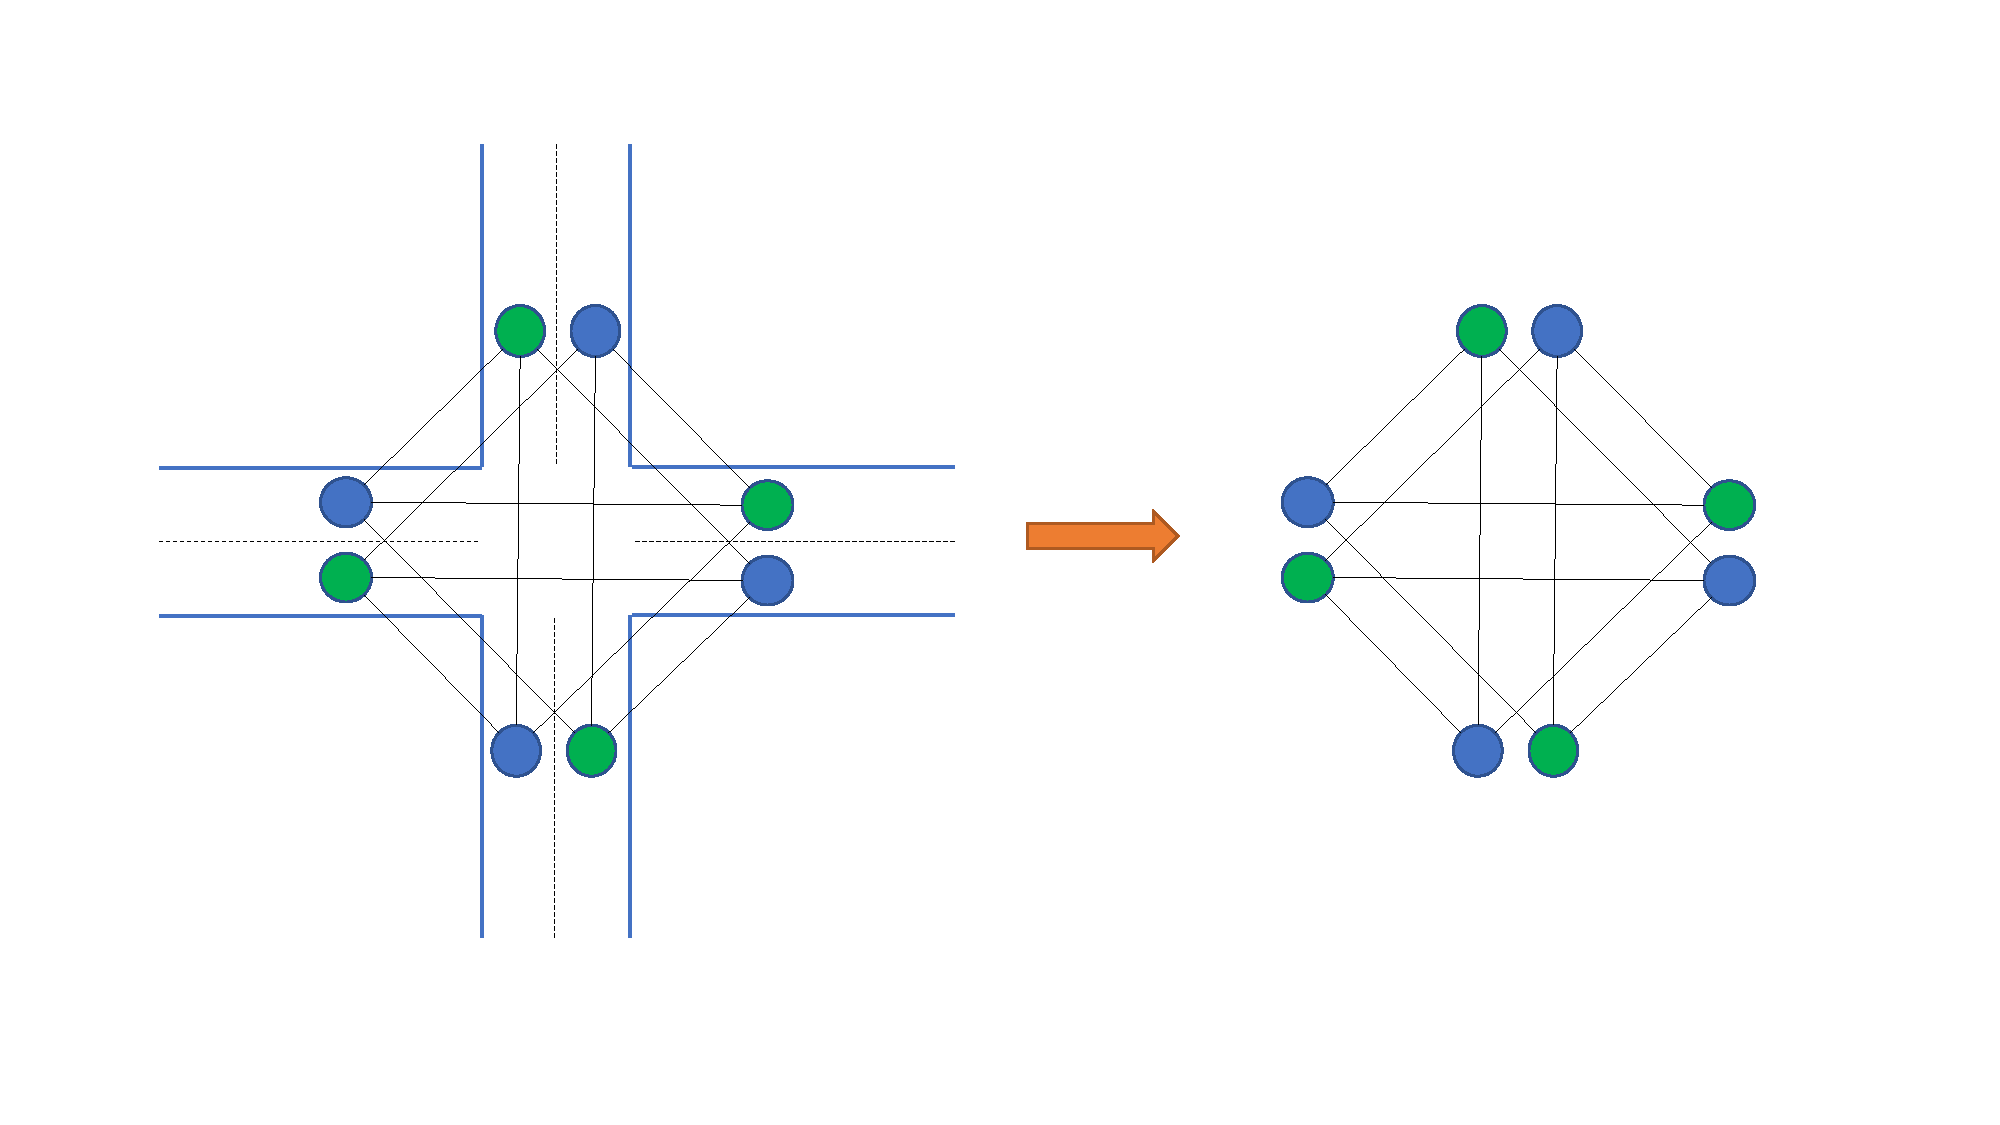
\includegraphics[width=12cm]{ppt/graph-modeling.pdf}
  \caption{按道路建模成图}
  \label{fig:network-graph-new}
\end{figure}

然后我们将相位信息加入到图的结构信息中,这里我们规定边有一个权重值$WE$,如果在当前相位下,道路i到道路j之间是允许通行的,则连接这两个节点的边的权重$WE_{ij}=1$,如果不允许通行,
则$WE_{ij}=0$。这个权重将用作后续剔除信息无关节点(该节点的信息对目标节点没有影响)。


这里我们使用注意力机制(Attention Mechanism)学习来学习邻近节点的表示对目标节点状态的影响,从而实现通信的目的。整个过程可以分解为以下几个步骤:

1. 观察交互(Observation Interaction)
为了了解来自路口j(源节点)的信息在确定路口i(目标节点)的策略的重要性,我们首先嵌入(Embedding)来自前一层的这两个节点的表示并用来计算$e_{ij}$(在确定路口i的策略时路口j的重要性),
按照下列的操作:
\begin{align}
\label{eq:eij}
  e_{ij}=(h_i W_t) \dot (h_j W_s)^{T},
\end{align}

其中$W_s, W_t \in \mathbf{R}^{mxn}$分别是源节点和目标节点的嵌入参数。值得注意的是,这里$e_{ij}$不一定等于$e_{ji}$。例如,

2. 无关信息剔除
\begin{align}
  \label{eq:mul_phase}
  e_{ij} = e_{ij} * WE_{ij},
\end{align}
这里$WE_{ij}$是连接i和j的边的权重。

3. 计算邻域范围的注意力分布
为了获取目标节点和源节点之间的注意力值,我们将目标节点及其邻近节点之间的互动分数(即,$e_{ij}$)进行归一化:
% \begin{align}
%   \label{eq:attention}

% \end{align}


